%%  Chapter 3 - Data and Methodology
\ifpdf
\graphicspath{{Chapter3/Figs/Raster/}{Chapter3/Figs/PDF/}{Chapter3/Figs/}}
\else
\graphicspath{{Chapter3/Figs/Vector/}{Chapter3/Figs/}}
\fi

\chapter{Data and Methodology}
\label{ch:methodology}

\section{Data Sources}
\label{sec:data_sources}

\subsection{ERA5 Reanalysis}
\label{subsec:era5}

The primary dataset is the ERA5 global reanalysis produced by the
European Centre for Medium-Range Weather Forecasts (ECMWF)
\citep{hersbach2020era5}. ERA5 provides hourly estimates of
atmospheric, land-surface, and oceanic variables on a regular
latitude-longitude grid at $0.25^\circ \times 0.25^\circ$ horizontal
resolution (approximately 28\,km at the equator), with 37 pressure
levels from 1000\,hPa to 1\,hPa. The dataset is generated through a
4D-Var data assimilation system that ingests conventional and
satellite observations \citep{hersbach2020era5}.

The following ERA5 surface and single-level fields are used at hourly
temporal resolution over the domain 5-35$^\circ$N, 60-100$^\circ$E:

\begin{itemize}
  \item \textbf{850\,hPa relative vorticity} (\texttt{vo}): MD
    detection, tracking, and centre identification.
  \item \textbf{Mean sea-level pressure} (\texttt{msl}):
    closed-circulation verification.
  \item \textbf{Surface latent heat flux} (\texttt{slhf},
    J\,m$^{-2}$, accumulated): de-accumulated to W\,m$^{-2}$;
    positive upward throughout.
  \item \textbf{Surface sensible heat flux} (\texttt{sshf},
    J\,m$^{-2}$, accumulated): de-accumulated identically.
  \item \textbf{Volumetric soil water layer\,1} (\texttt{swvl1},
    m$^3$\,m$^{-3}$): 0-7\,cm near-surface soil moisture, instantaneous.
  \item \textbf{Total precipitation} (\texttt{tp}, m\,hr$^{-1}$,
    accumulated): de-accumulated to mm\,hr$^{-1}$.
  \item \textbf{2-m dewpoint temperature} (\texttt{d2m}, K):
    boundary-layer moisture saturation state.
  \item \textbf{2-m temperature} (\texttt{t2m}, K): surface thermodynamic state.
  \item \textbf{Land-sea mask} (\texttt{lsm}): land/ocean
    classification (\texttt{lsm} $\geq 0.5$ = land).
  \item \textbf{10-m U and V wind components}: translational flow environment.
\end{itemize}

ERA5 accumulated flux variables are de-accumulated to instantaneous values as:
\begin{equation}
  F_\mathrm{inst}(t) = \frac{F_\mathrm{acc}(t) - F_\mathrm{acc}(t -
  1\,\mathrm{h})}{\Delta t_s},
  \label{eq:deaccumulate}
\end{equation}
where $F_\mathrm{acc}$ is the accumulated value in J\,m$^{-2}$ and
$\Delta t_s = 3600$\,s. ERA5 uses a sign convention in which LHF is
negative upward; this convention is corrected throughout so that
positive values denote upward flux.

\subsection{IMD Monsoon Seasonal Reports}
\label{subsec:imd_data}

The India Meteorological Department (IMD) publishes annual Monsoon
Seasonal Reports providing synoptic track information for all LPS
over the north Indian Ocean, including formation date, landfall time,
landfall location, and dissipation time. These reports are used to
cross-validate ERA5-derived MD tracks.

\subsection{SRTM Elevation Data}
\label{subsec:srtm}

Shuttle Radar Topography Mission (SRTM) 1-arc-second ($\approx
30$\,m) DEM tiles in HGT format are used for terrain
characterisation. Tiles are loaded and interpolated to track
positions by bilinear interpolation.

\section{Study Domain and Period}
\label{sec:domain}
% FULL_EXTENT = [70.0, 95.0, 7.0, 30.0]  # lon_min, lon_max, lat_min, lat_max

The analysis covers June-September for 2001-2025. The ERA5 extraction
domain is 7-30$^\circ$N, 70-95$^\circ$E.

%%  FIGURE: Study domain map
%%  Show ERA5 domain box, detection domain box (inner), Eastern Ghats
% contours, BoB, and preferred landfall zone
\begin{figure}[h]
  \centering
  % \fbox{\rule{0pt}{7cm}\rule{0.85\textwidth}{0pt}}
  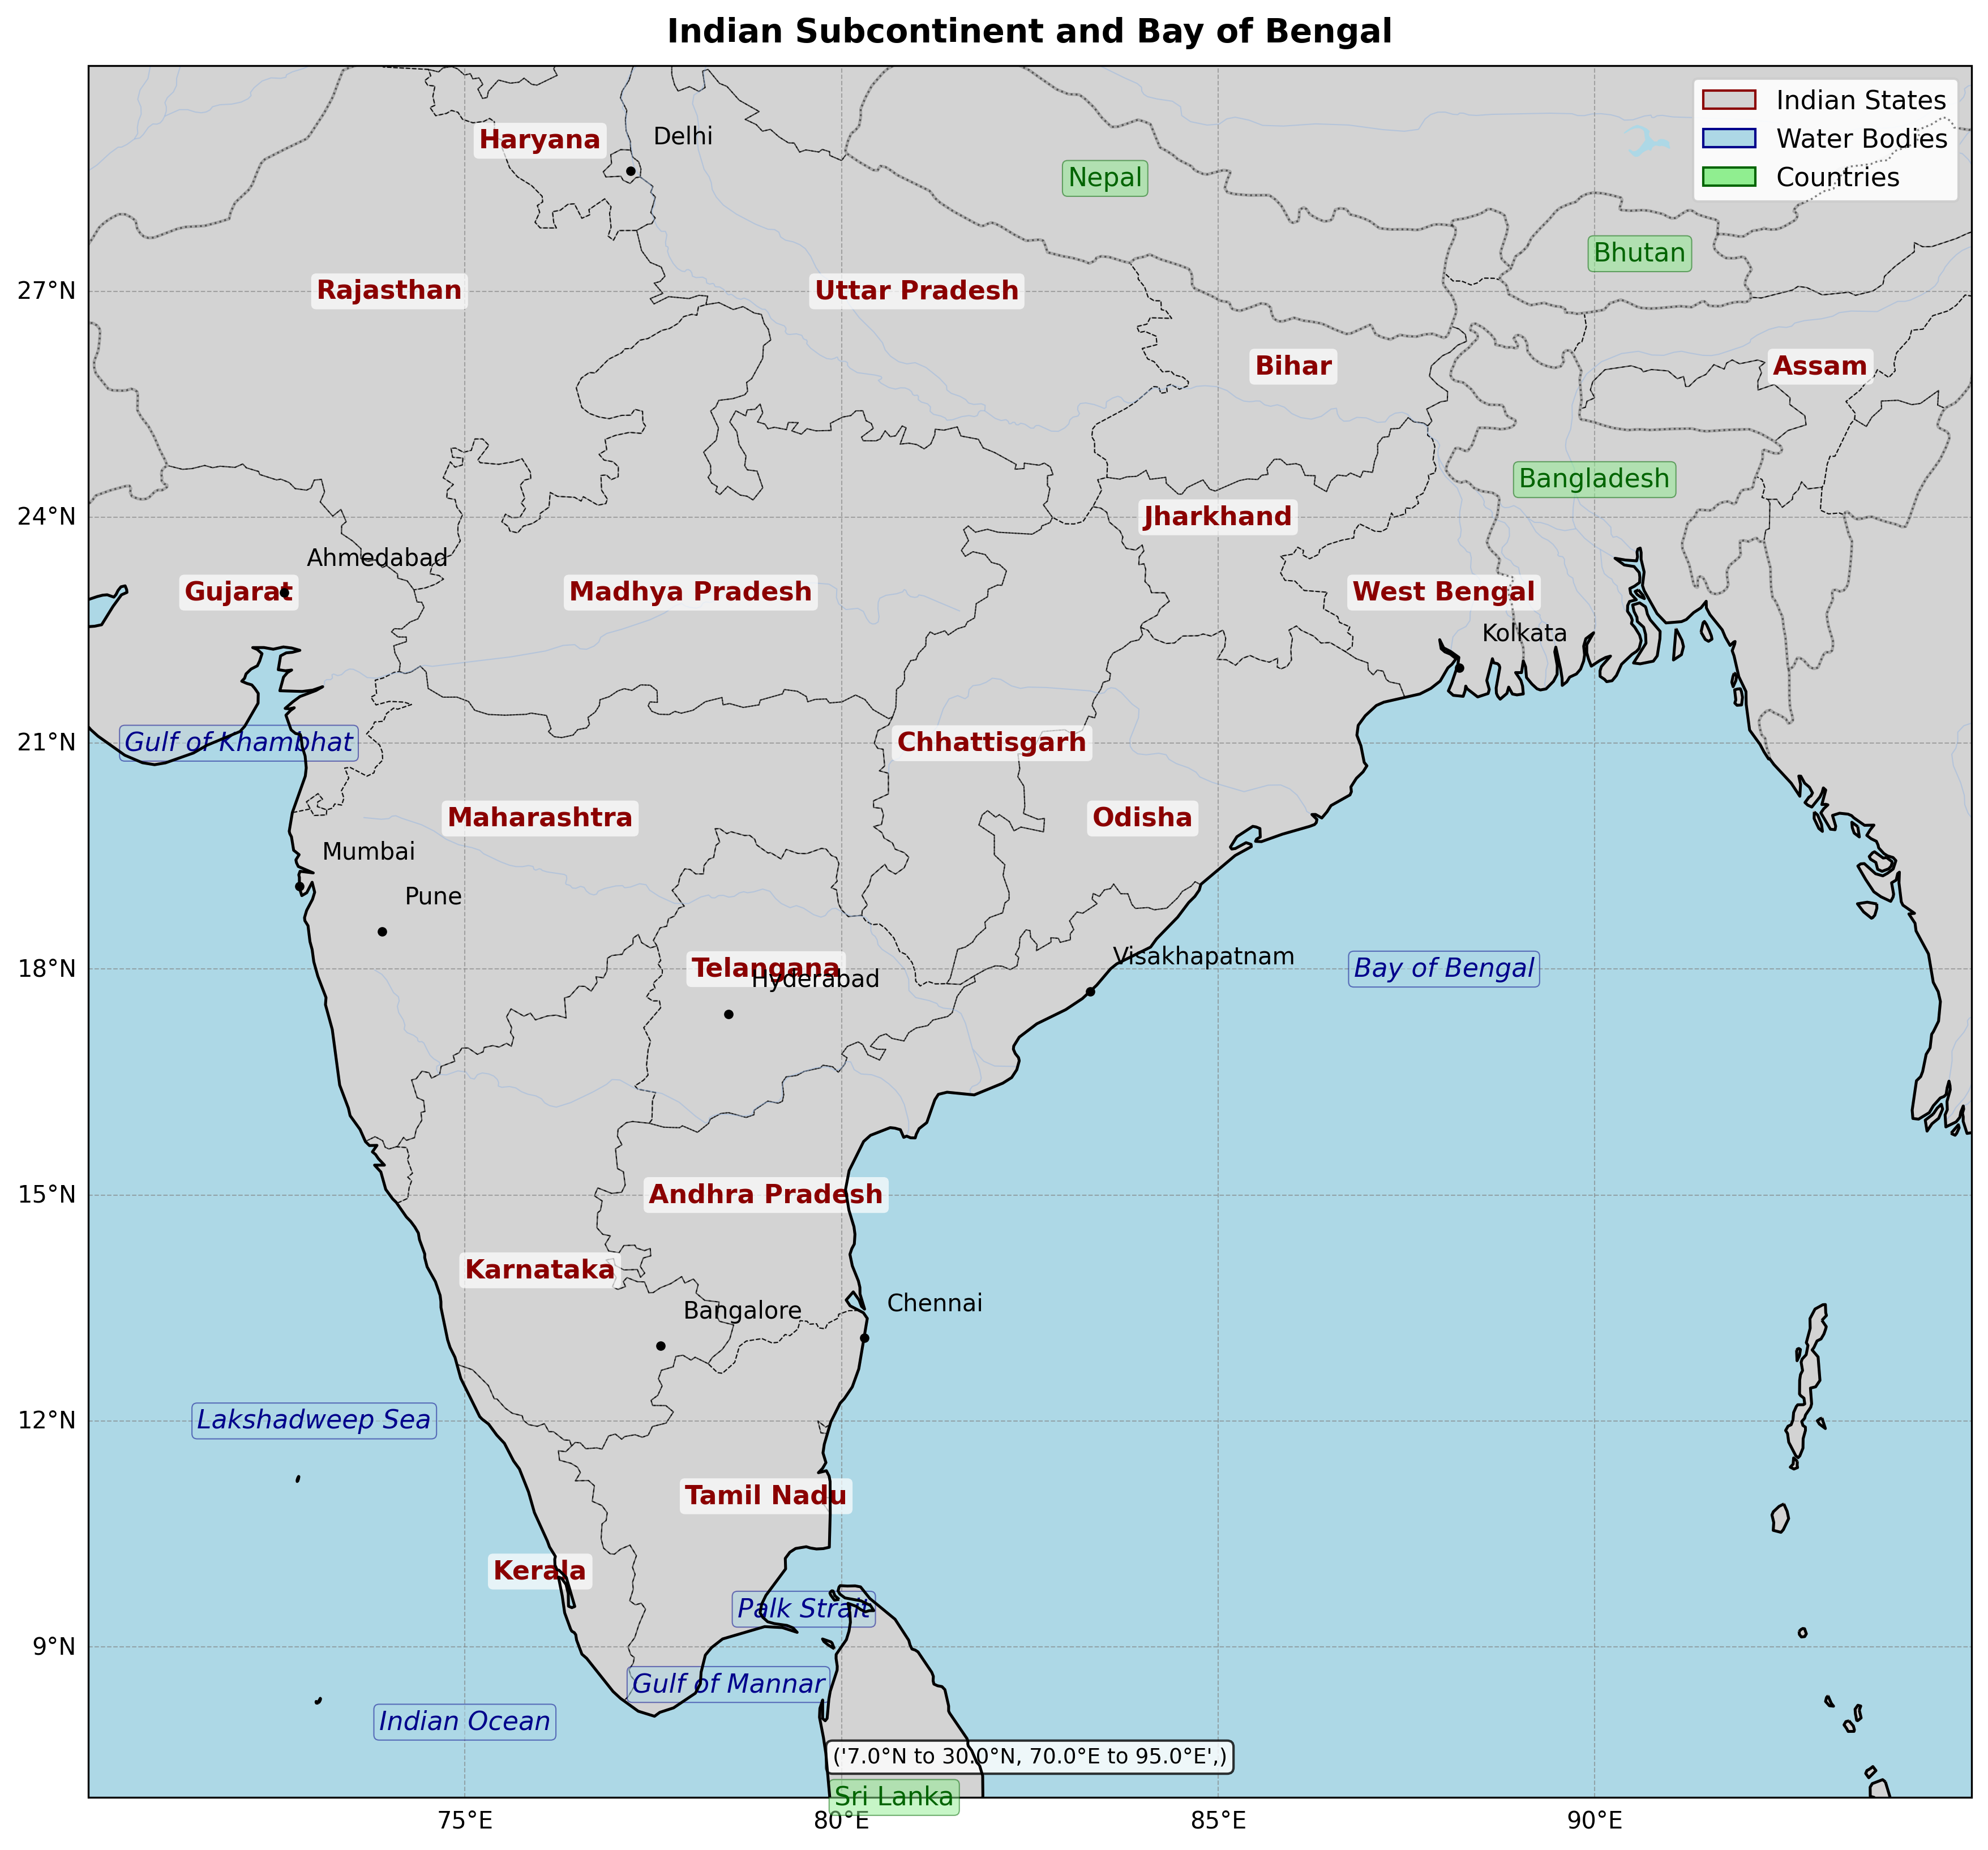
\includegraphics[width=0.85\textwidth]{Chapter3/Figs/study_domain_detailed_labels.png}
  \caption[Study domain and ERA5 analysis region]{Study domain for ERA5 analysis
  (7-30$^\circ$N, 70-95$^\circ$E).}
  \label{fig:study_domain}
\end{figure}

\section{Monsoon Depression Detection and Tracking}
\label{sec:md_detection}

\subsection{Detection Algorithm}
\label{subsec:detection}

MD detection operates on hourly ERA5 850\,hPa relative vorticity using a
threshold-based approach implemented in \texttt{md\_detect.py}:

\begin{enumerate}
  \item \textbf{Vorticity thresholding}: $\zeta_{850} \geq 4.0 \times
    10^{-5}$\,s$^{-1}$.
  \item \textbf{Local maximum detection}: maxima within a $3^\circ
    \times 3^\circ$ neighbourhood are retained.
  \item \textbf{Closed circulation check}: MSLP within 400\,km radius
    must show a closed cyclonic isobar.
  \item \textbf{Persistence filter}: threshold must be sustained for
    at least 12 consecutive hours.
  \item \textbf{Domain restriction}: track predominantly within
    10-30$^\circ$N, 70-95$^\circ$E.
\end{enumerate}

\subsection{Track Construction and Land-Sea Classification}
\label{subsec:tracking}

Consecutive maxima are linked by nearest-neighbour search with
maximum displacement $5^\circ$ per 6\,h. Land/ocean classification
uses \texttt{lsm} $\geq 0.5$ = land. Landfall is the first
land-classified point after $\geq 2$ consecutive ocean points.

%%  FIGURE: Detection algorithm flowchart
%%  SUGGESTED SOURCE: Draw in draw.io, Inkscape, or using Python's
% matplotlib patches.
%%  Show boxes: ERA5 Input -> Vorticity Threshold -> Local Max ->
% Closed Circ Check
%%  -> Persistence Filter -> Domain Check -> Track Output -> IMD Validation.
\begin{figure}[ht]
  \centering
  %% >> INSERT FIGURE: Chapter3/Figs/detection_flowchart.pdf <<
  %% (Flowchart: ERA5 vorticity -> threshold -> local max -> MSLP check ->
  %%  persistence filter -> IMD cross-validation -> confirmed MD track)
  \fbox{\rule{0pt}{9cm}\rule{0.75\textwidth}{0pt}}
  % \includegraphics[width=0.75\textwidth]{Chapter3/Figs/detection_flowchart}
  \caption[MD detection algorithm flowchart]{Flowchart of the ERA5-based MD
  detection and tracking algorithm.}
  \label{fig:detection_flowchart}
\end{figure}

\subsection{IMD Cross-Validation and Duration Classification}
\label{subsec:imd_validation}

ERA5 tracks are matched to IMD records using formation date ($\pm 24$\,h) and
landfall location ($\pm 2^\circ$). Systems are classified as \emph{short-lived}
($< 96$\,h) or \emph{long-lived} ($\geq 96$\,h).

\section{Rationale for the Azimuthal Hovm\"{o}ller Framework}
\label{sec:hovmoller_rationale}

A central methodological challenge in diagnosing land-surface on a
\emph{moving} system is separating the local storm-scale signal from
the background gradient. Fixed-grid analyses of ERA5 latent heat flux
soil moisture India superimpose several confounding signals
simultaneously: seasonal north-south in soil moisture, the spatial
gradient in net radiation, and large-scale moisture advection. These
signals are spatially coherent on comparable the MD itself, making it
impossible to isolate the storm-induced anomaly.

The Azimuthal Hovm\"{o}ller approach addresses this problem by
re-expressing all in a coordinate system that \emph{moves with the MD
}. At each time , the analysis domain is re-centred on the current
track , and all variables expressed as azimuthally averaged radial
profiles relative to the centre.

This has three critical advantages:
\begin{enumerate}
  \item \textbf{Background gradient removal.} The radial coordinate
    measures distance \emph{from the storm centre}, not geographic
    position. Systematic north-south or east-west gradients in soil
    moisture or flux therefore appear as uniform offsets in the
    radial coordinate rather than as spurious radial structure.
  \item \textbf{Time-space coherence.} The Hovm\"{o}ller diagram
    places time (including the critical landfall transition) on one
    axis and radial distance on the other, enabling direct
    before-and-after comparison at every radius simultaneously.
  \item \textbf{Separation of inner-core from outer-band signals.}
    The radial dimension cleanly separates inner-core processes ($r <
    100$\,km, driven by surface energy flux and organised convection)
    from outer-band processes ($r = 100-400$\,km, driven by
    large-scale moisture advection), which is critical for isolating
    the BOE signature.
\end{enumerate}

\subsection{Construction of the Azimuthal Hovm\"{o}ller: Step-by-Step}
\label{subsec:hovmoller_construction}

The azimuthal averaging procedure is illustrated in
~\ref{fig:hovmoller_geometry} proceeds as follows at each time step
$t$ with track centre at latitude-longitude $(\phi_c, \lambda_c)$:

\paragraph{Step 1: Radial Binning.}
For every ERA5 grid point within 400\,km of the track centre, the
circle distance $r$ is computed using the Haversine formula:
\begin{equation}
  r = 2R_E \arcsin\!\sqrt{\sin^2\!\frac{\Delta\phi}{2} +
  \cos\phi_c\cos\phi\,\sin^2\!\frac{\Delta\lambda}{2}},
  \label{eq:haversine}
\end{equation}
where $R_E = 6371$\,km, and $\Delta\phi$, $\Delta\lambda$ are the
latitude and longitude separations from the centre. Each grid point
is assigned to one of 16 radial bins: $r \in [0, 25),\,[25,
50),\,\ldots,\,[375, 400)$\,km, each of width 25\,km.

\paragraph{Step 2: Azimuthal Sectoring.}
Within each radial bin, the 360$^\circ$ azimuth is divided into 16
equal sectors of $22.5^\circ$ each (N, NNE, NE, ENE, E, \ldots, NNW).
Grid points are assigned to sectors by their bearing from the storm centre:
\begin{equation}
  \theta = \arctan2(\Delta\lambda \cos\phi_c,\; \Delta\phi).
  \label{eq:bearing}
\end{equation}
This divides the storm domain into $16 \times 16 = 256$
sector-annulus segments (Figure~\ref{fig:hovmoller_geometry}).

\paragraph{Step 3: Sector Averaging.}
For each of the 16 sectors within a given radial bin, the mean value
of the target variable (LHF, precipitation, \texttt{swvl1}, etc.) is
computed from all ERA5 grid in that sector. This yields 16
sector-mean values per radial per time step.
These 16 values are then averaged (equally weighted) to produce a
radial-mean at radius $r$ at time $t$.

\paragraph{Step 4: Hovm\"{o}ller Assembly.}
Repeating Steps 1-3 for all time steps $t = 1, \ldots, T$ produces
Hovm\"{o}ller $H(r, t)$ of dimensions $16 \times T$. The $x$-axis is
time (aligned to at $t=0$; negative values = ocean phase; positive
values = land phase); $y$-axis is radial distance (0-400\,km from
storm centre). This matrix is as a colour-filled contour diagram for
each variable.

% FIGURE: Azimuthal Hovmoller geometry
\begin{figure}[h]
  \centering
  %% (Polar plot: concentric rings at 25km intervals to 400km, 16
  % sectors at 22.5deg,
  % \fbox{\rule{0pt}{7.5cm}\rule{0.75\textwidth}{0pt}}
  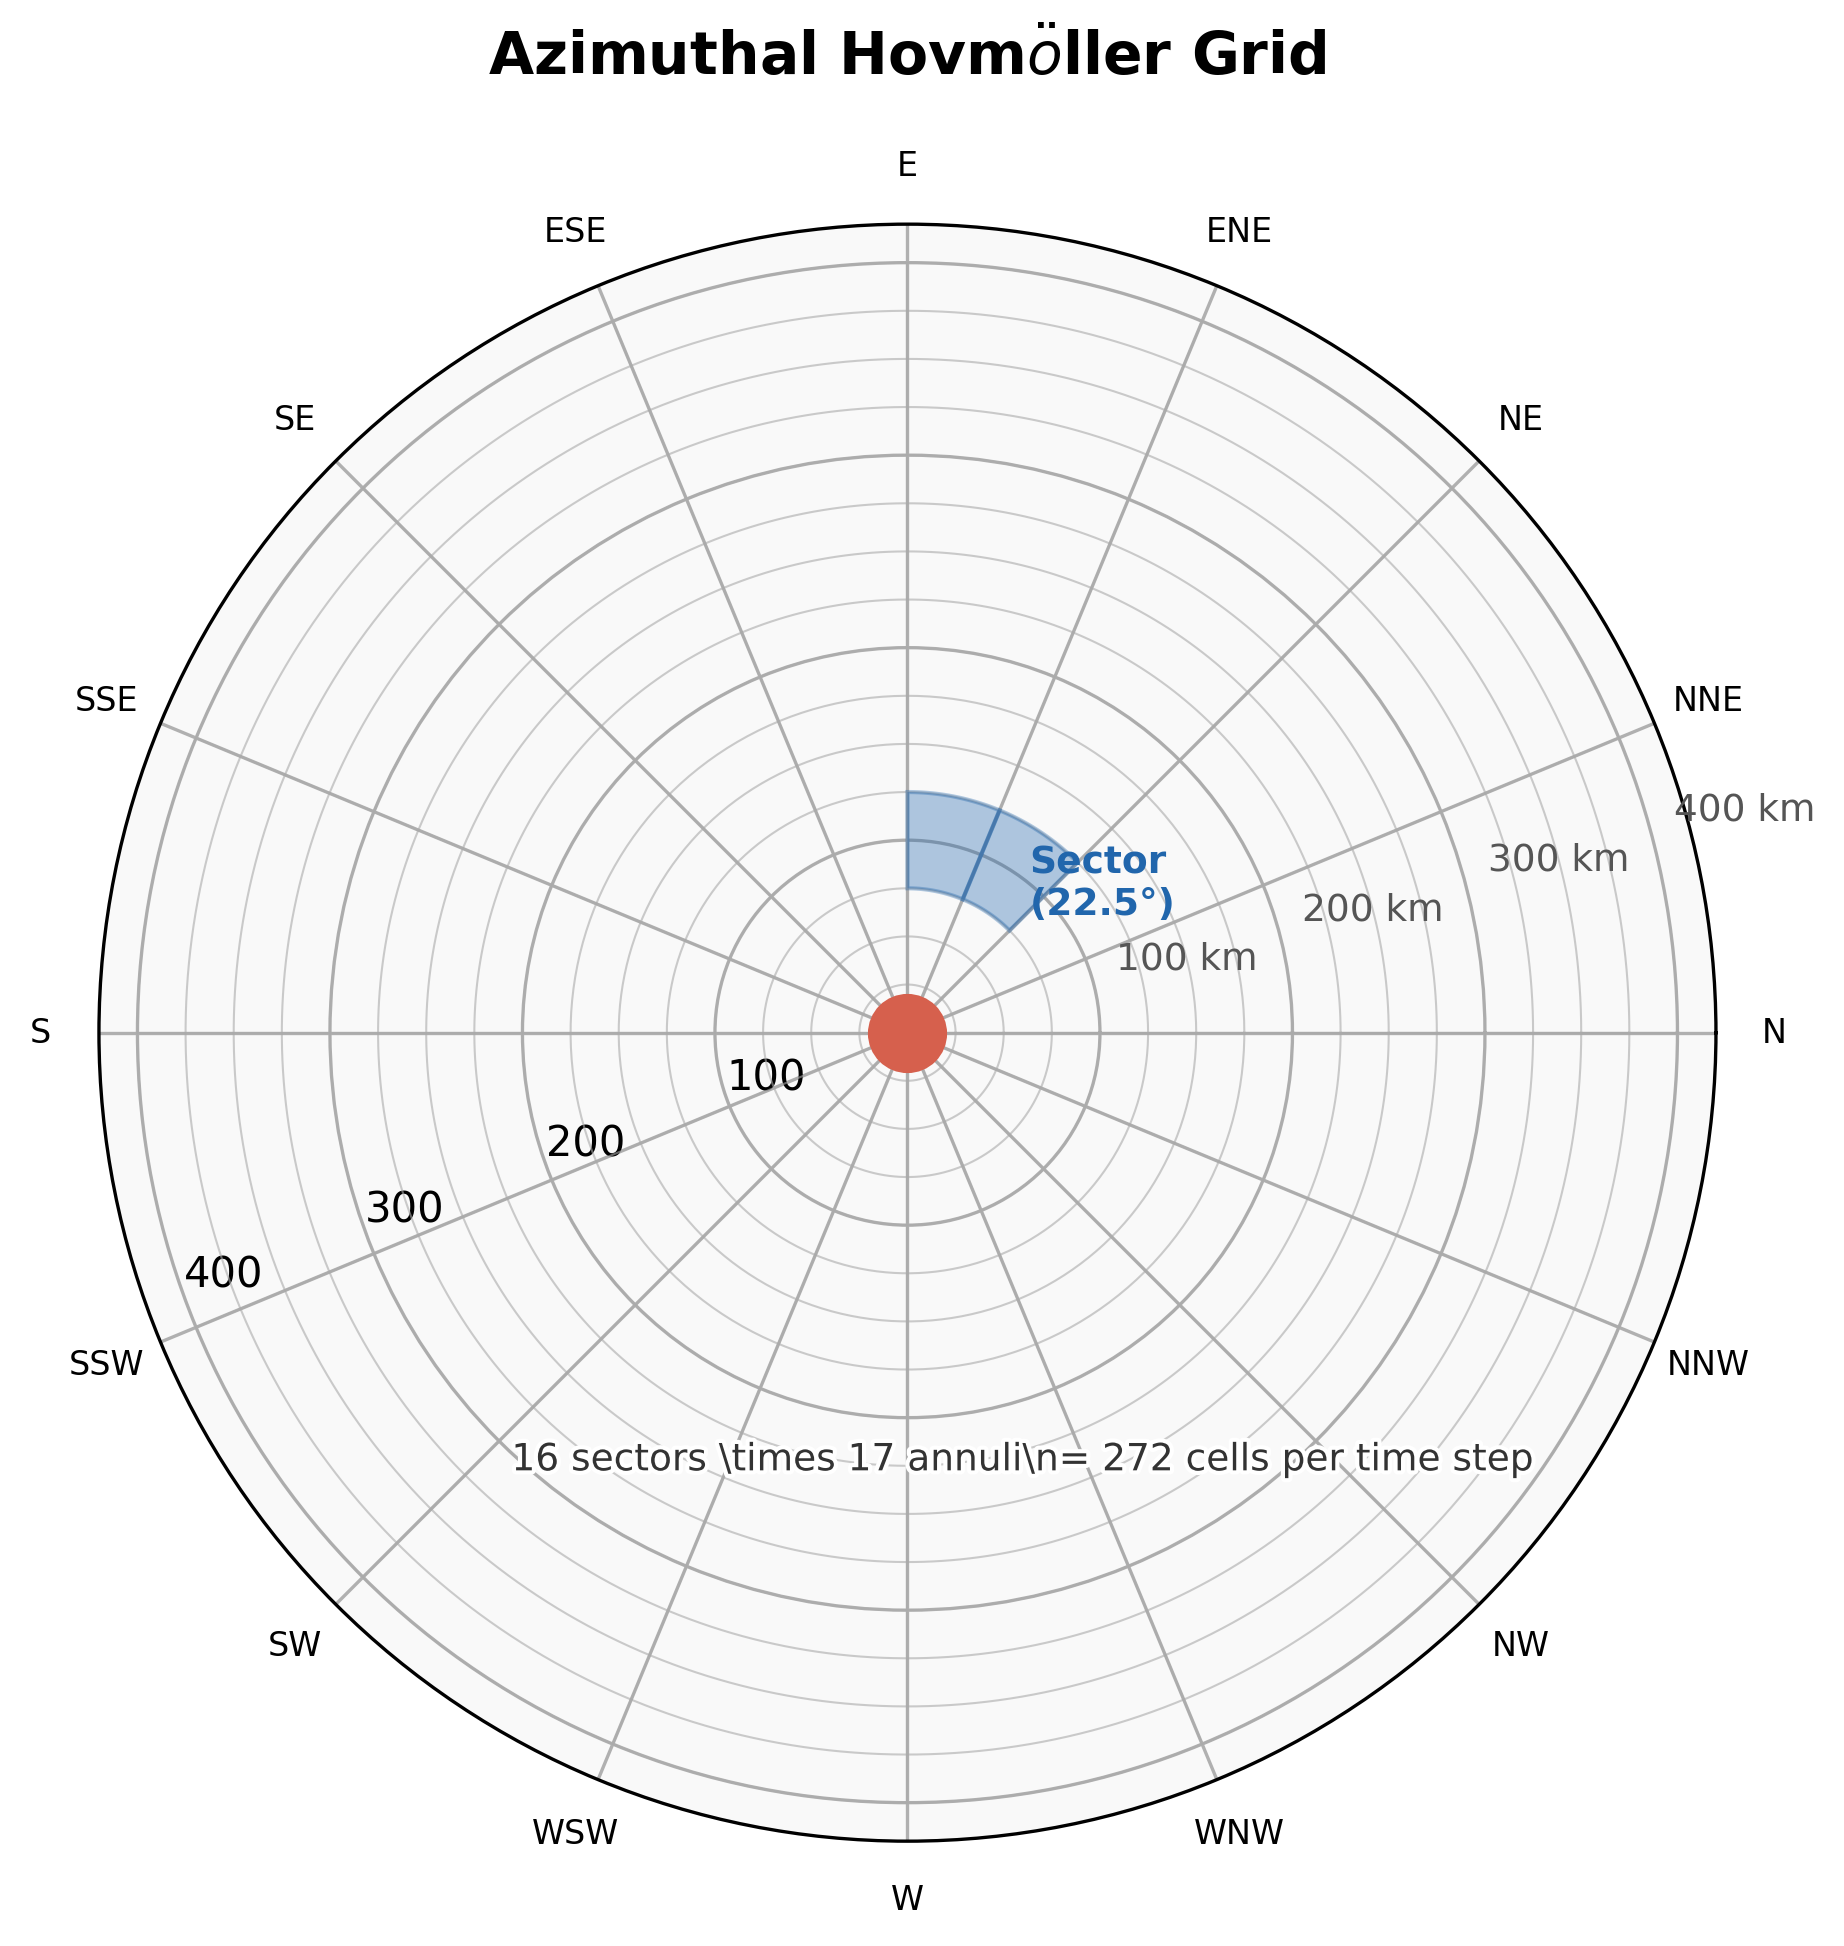
\includegraphics[width=0.75\textwidth]{Chapter3/Figs/hovmoller_geometry.png}
  \caption[Azimuthal Hovm\"{o}ller radial binning geometry]{Polar grid for the
    Azimuthal Hovm\"{o}ller construction. The MD centre is surrounded by
    concentric rings at 25\,km intervals to 400\,km, divided into 16 sectors of
    22.5$^\circ$ each. All ERA5 grid points in each sector-annulus
    cell are averaged;
    the 16 sector values are then azimuthally averaged to produce the
    radial profile
  at each time step.}
  \label{fig:hovmoller_geometry}
\end{figure}

%%  FIGURE: Example Hovmoller output annotated
%%  Annotate with: landfall dashed line, inner core zone (<100km),
% outer band zone, ocean phase label, land phase label.
\begin{figure}[h]
  \centering
  %% (An example LHF Hovmoller: annotate t=0 landfall line, radial
  % zones, phase labels)
  % \fbox{\rule{0pt}{6.5cm}\rule{0.85\textwidth}{0pt}}
  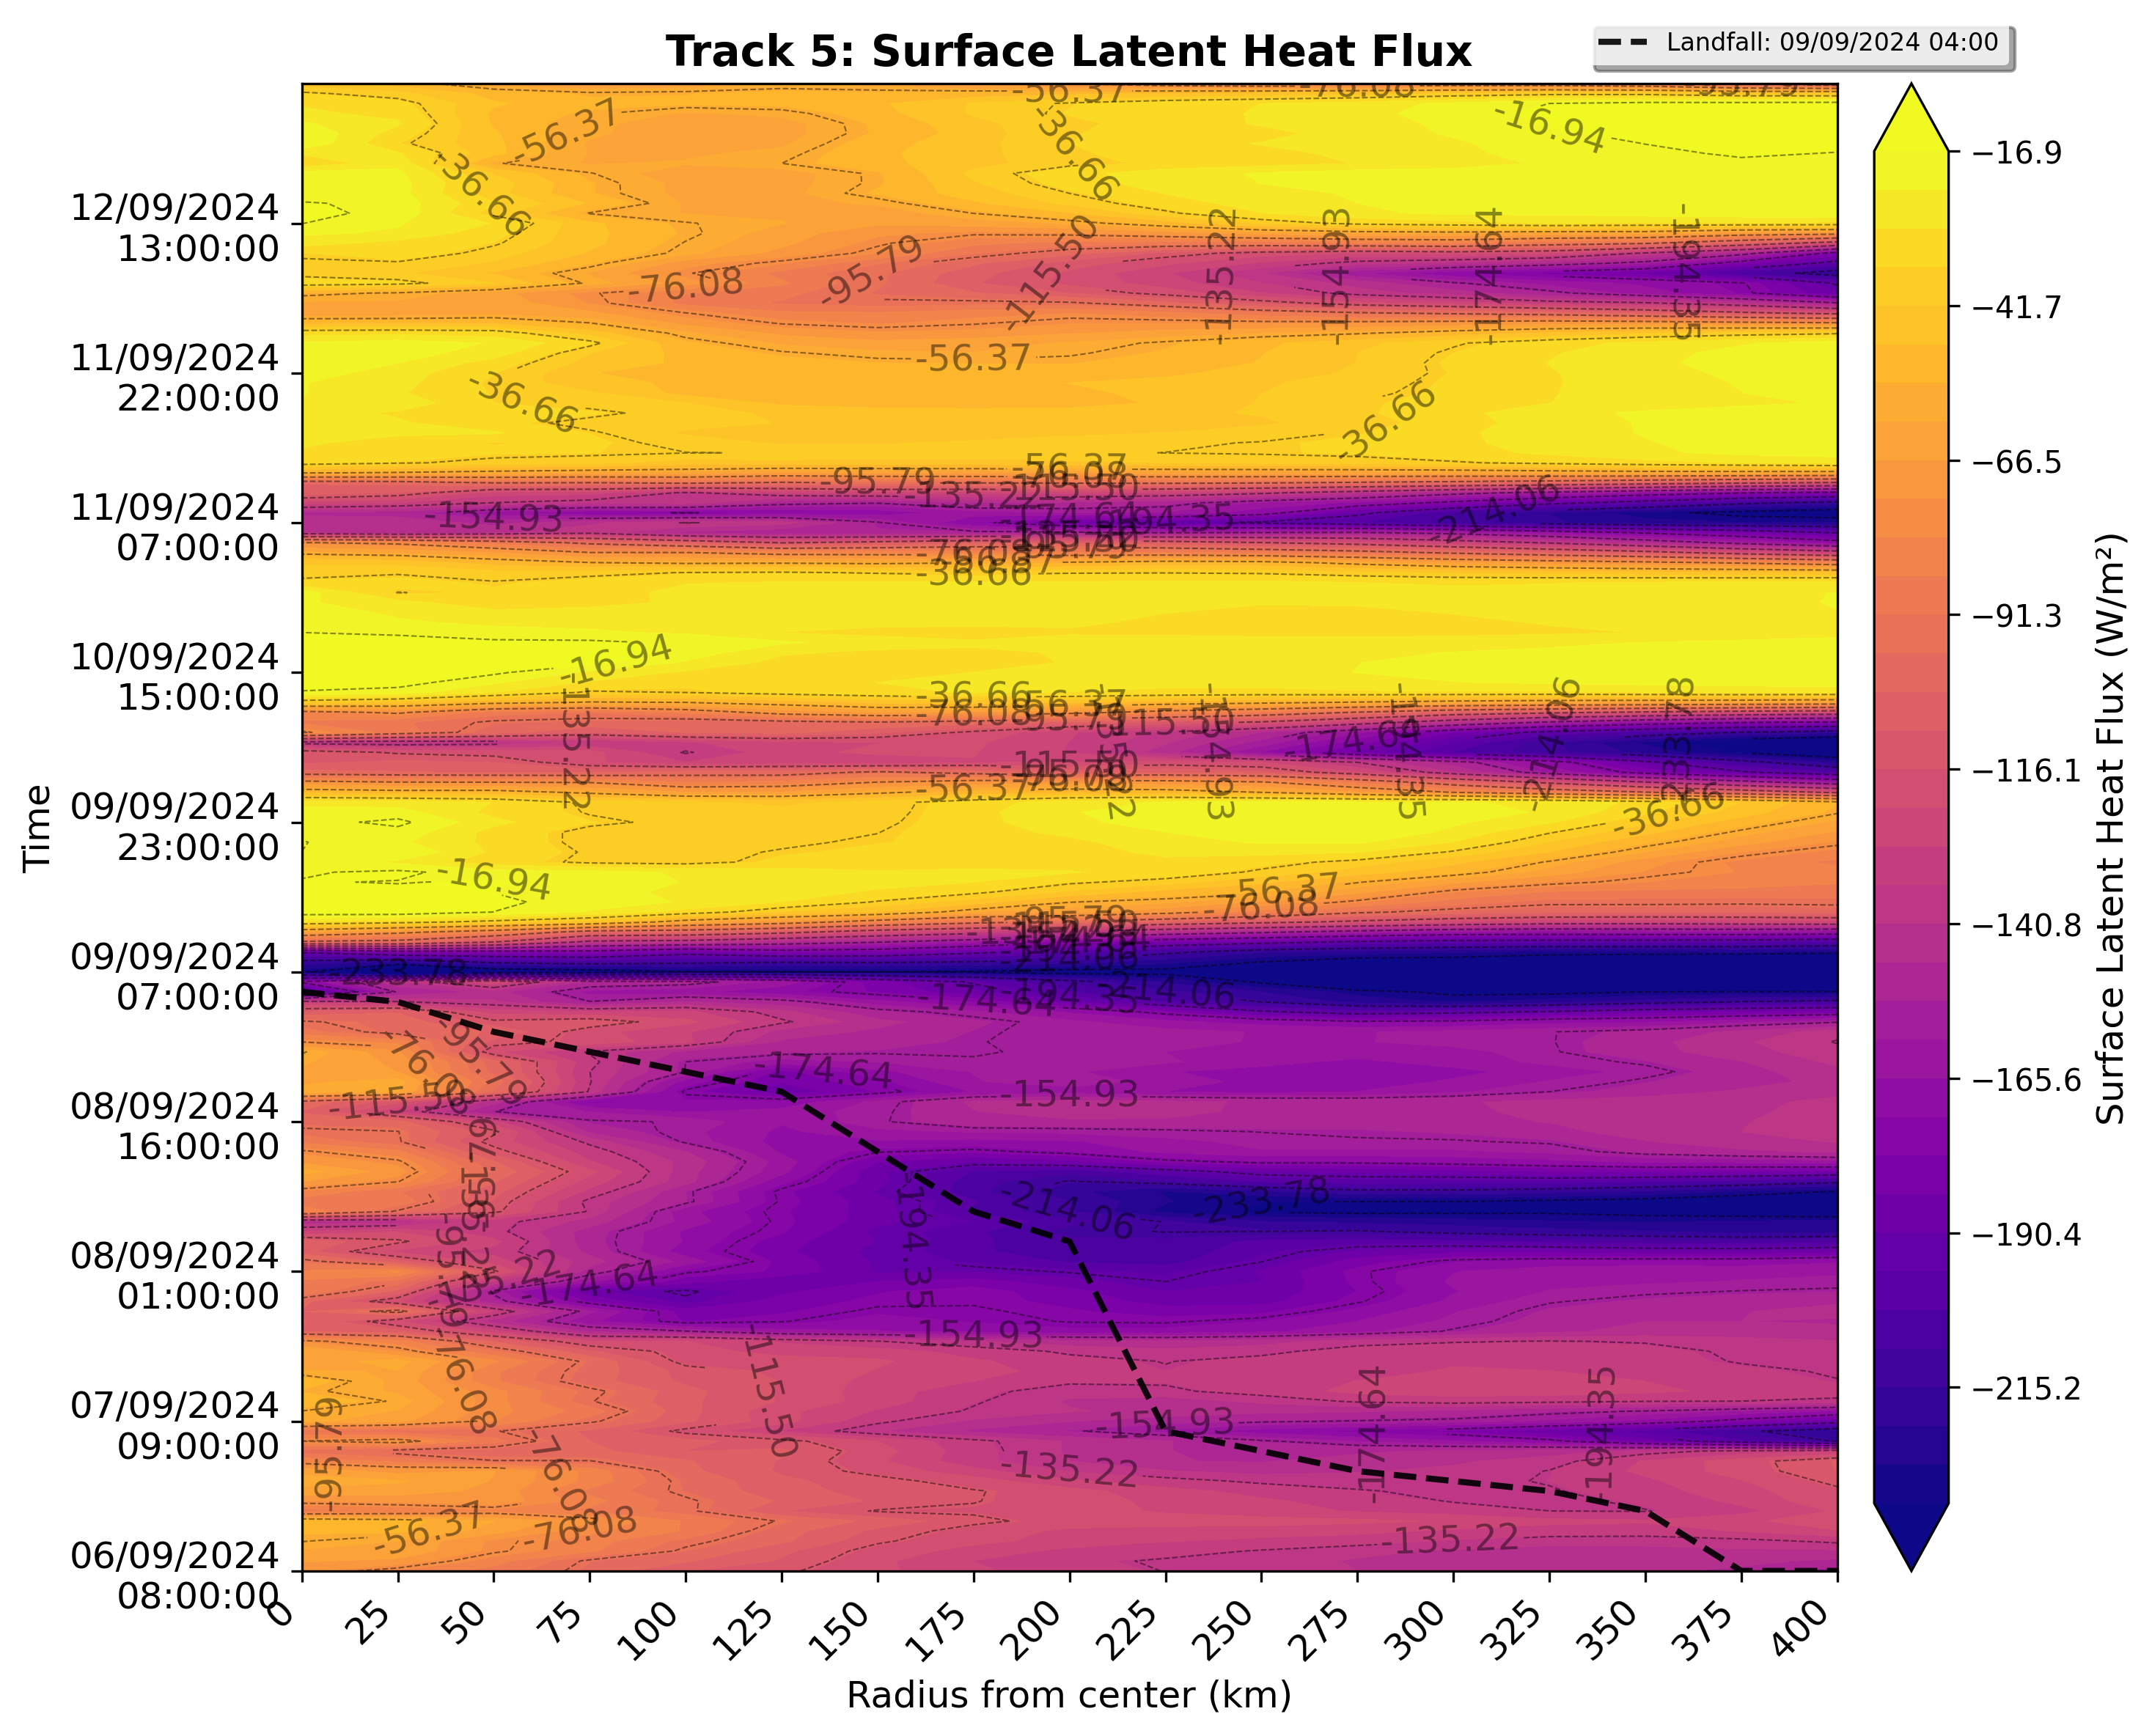
\includegraphics[width=0.85\textwidth]{Chapter3/Figs/hov_avg_slhtf_azimuthal_avg.png}
  \caption[Example annotated Azimuthal Hovm\"{o}ller (LHF)]{Example Azimuthal
    Hovm\"{o}ller of surface LHF (W\,m$^{-2}$) for a representative
    long-lived MD.
    The dashed line marks landfall. Ocean phase and land phase are separated
  at the dashed line.}
  % Inner core ($r < 100$\,km) and outer band ($r = 100-400$\,km)
  % zones are labelled.
  \label{fig:hovmoller_example}
\end{figure}

\subsection{Variables Computed in the Hovm\"{o}ller Framework}
\label{subsec:hovmoller_variables}

Six variables are computed: total precipitation (mm\,hr$^{-1}$),
surface LHF W\,m$^{-2}$), surface SHF (W\,m$^{-2}$), near-surface
soil moisture m$^3$\,m$^{-3}$), 2-m dew-point depression ($T_{2m} -
T_{d,2m}$, K), and soil tendency (m$^3$\,m$^{-3}$\,hr$^{-1}$).

\section{Track-Following Time-Series Diagnostics}
\label{sec:timeseries_method}

Track-following time series extract spatially averaged values within
100\,km buffer on the track position at each time step. All time
series are aligned to ($t = 0$). Variables are stratified by
land/ocean classification. Following diagnostic outputs for each confirmed MD:

\yellownote{CHECK this}
\begin{description}
\item[\texttt{track\_N\_HF\_time\_series.png}]
Time series of surface LHF, SHF, and total heat flux centred on landfall,
with ocean/land phase shading. Primary plot for BOE candidate
identification.
\item[\texttt{track\_N\_TP-SWVL1\_time\_series.png}]
Dual-axis time series of \texttt{swvl1} and total precipitation, showing
co-evolution of surface moisture state and rainfall.
\item[\texttt{track\_N\_bowen\_ratio.png}]
Time series of the Bowen ratio $\beta = Q_H / Q_E$, quantifying the
land-phase shift in surface energy partitioning.
\item[\texttt{track\_N\_theta\_e\_timeseries.png}]
Equivalent potential temperature $\theta_e$ at the inner-core region
(0-100\,km), tracking boundary-layer thermodynamic stability.
\item[\texttt{track\_N\_dpd\_windward\_leeward.png}]
Dew-point depression computed separately for windward (eastern) and leeward
(western) sectors of the Eastern Ghats, diagnosing boundary-layer moisture
asymmetry.
\item[\texttt{track\_N\_recycling\_ratio.png}]
Precipitation recycling ratio $\rho$, quantifying the fraction of
precipitation
sourced from local surface evapotranspiration vs large-scale advection.
\item[\texttt{track\_N\_diurnal\_HF\_amplitude.png}]
Diurnal amplitude of the sensible heat flux. A small SHF diurnal amplitude
indicates a moist surface suppressing daytime sensible heating.
\end{description}

\section{Surface Heat Flux Analysis and BOE Classification}
\label{sec:heatflux_method}

For each land-falling MD, the 24-hour mean LHF, SHF, and total flux
are computed the windows immediately before and after landfall. A
system is classified as BOE candidate if:
\begin{equation}
\text{LHF}_\text{land} \geq 70\,\text{W\,m}^{-2}
\quad \text{for} \geq 18\,\text{consecutive hours.}
\label{eq:boe_criterion}
\end{equation}

\section{Antecedent Soil Moisture Index}
\label{sec:asmi_method}

The ASMI is an exponentially weighted temporal average of
texttt{swvl1} over the inland track corridor:
\begin{equation}
\text{ASMI}(L) =
\frac{\sum_{d=1}^{L} e^{-\kappa(d-1)}\,\bar{S}_d}
{\sum_{d=1}^{L} e^{-\kappa(d-1)}},
\label{eq:asmi}
\end{equation}
with decay constant $\kappa = 0.85$. Lag windows of 24\,h, 3\,d,
7\,d, and 14\,d computed. The exponential weighting means that more
recent soil moisture contribute more than older conditions,
consistent with the physical that moisture memory decays with time.

\section{Translational Speed and Terrain Characterisation}
\label{sec:speed_terrain_method}

Translational speed is computed from consecutive Haversine distances
by the interval (Section~\ref{sec:asmi_method}. The Terrain
Sensitivity Index (TSI) at each track point combines normalised
elevation contrast ($E^*$), slope ($S^*$), and roughness ($R^*$) from
the SRTM DEM:
\begin{equation}
\text{TSI} = E^* \times S^* \times R^*.
\label{eq:tsi}
\end{equation}
A high TSI indicates a complex, steep, rough terrain zone likely to
decelerate the MD and disrupt its circulation structure.

\section{Summary of Methodological Workflow}
\label{sec:method_summary}

%%  FIGURE: Methodological workflow
%%  SUGGESTED SOURCE: Draw in draw.io, Lucidchart, or PowerPoint.
%%  Boxes: ERA5 -> MD Detection -> IMD Validation -> Track DB ->
%%  [Hovmoller | Time Series | ASMI | Terrain] -> BOE Classification
% -> Statistics
\begin{figure}[h]
\centering
%% >> INSERT FIGURE: Chapter3/Figs/method_workflow.pdf <<
%% (Flowchart: ERA5 + SRTM inputs -> detection -> four parallel
% analysis streams
%%  -> BOE classification and statistical output)
\fbox{\rule{0pt}{8.5cm}\rule{0.82\textwidth}{0pt}}
% \includegraphics[width=0.82\textwidth]{Chapter3/Figs/method_workflow}
\caption[Overall methodological workflow]{Complete methodological
  workflow. ERA5 hourly fields feed the MD detection algorithm,
  producing a validated track database. Each track feeds four parallel
  analysis streams: Azimuthal Hovm\"{o}ller diagnostics;
  track-following time-series; antecedent soil moisture index; and
  terrain characterisation via SRTM. All streams converge in the BOE
and statistical analysis stage.}
\label{fig:method_workflow}
\end{figure}

\begin{table}[h]
\centering
\caption[Summary of ERA5 variables]{ERA5 variables, identifiers,
processed units, analysis roles.}
\label{tab:variables_summary}
\begin{tabular}{l l l l}
  \toprule
  \textbf{Variable} & \textbf{ERA5 ID} & \textbf{Units} & \textbf{Role} \\
  \midrule
  850\,hPa relative vorticity & \texttt{vo}     &
  $10^{-5}$\,s$^{-1}$  & MD detection \\
  Mean sea-level pressure      & \texttt{msl}    & hPa
  & Circulation check \\
  Surface latent heat flux     & \texttt{slhf}   & W\,m$^{-2}$
  & BOE indicator \\
  Surface sensible heat flux   & \texttt{sshf}   & W\,m$^{-2}$
  & Energy partitioning \\
  Soil water (0-7\,cm)        & \texttt{swvl1}  & m$^3$\,m$^{-3}$
  & BOE, ASMI \\
  Total precipitation          & \texttt{tp}     & mm\,hr$^{-1}$
  & Feedback, Hovmöller \\
  2-m dewpoint temperature     & \texttt{d2m}    & K
  & BL moisture \\
  2-m temperature              & \texttt{t2m}    & K
  & Bowen ratio \\
  Land-sea mask                & \texttt{lsm}    & fraction
  & Phase classification \\
  \bottomrule
\end{tabular}
\end{table}
